\documentclass[conference]{IEEEtran}
\usepackage[utf8]{inputenc}
\usepackage[T1]{fontenc}
\usepackage{xcolor}
\usepackage{amsmath}
\usepackage{graphicx}
\usepackage{hyperref}
\graphicspath{ {./images/} } 

\begin{document}
\title{Game Playing Agent $|$ Minimax $|$ Alpha-Beta Pruning}
% author names and affiliations
\author{\IEEEauthorblockN{Vaishnav Mukesh}
\IEEEauthorblockA{202051196}
\and
\IEEEauthorblockN{Kaushik Rathva}
\IEEEauthorblockA{202051156}
\and
\IEEEauthorblockN{Patel Jaykumar}
\IEEEauthorblockA{202051136}
\and
\IEEEauthorblockN{Sontakke Ajinkya}
\IEEEauthorblockA{202051179}
}
% make the title area
\maketitle
\setlength{\parindent}{20pt}
\noindent Github link: \href{https://github.com/JARVIS-codebase/LAB-4}{LAB-4} \\ 
\indent To comprehend the Minimax algorithm and try to use alpha beta pruning to lower its time complexity. We shall discover that it is feasible to speed up processing and cut down on node assessments by trimming a few subtrees.\\ \\
\indent \begin{abstract}
Our objective is to use the Minimax algorithm on the game of noughts and crosses combined with improvisation utilising alpha beta pruning. Using the minimax value backup argument on the game tree, we also wish to illustrate that in the game of Nim, player 2 will always win regardless of the moves made by player 1.
\end{abstract}

\IEEEpeerreviewmaketitle

\section{Introduction}
\textbf{Playing Agent:} Playing agent in AI refer s to a computer program or sys tem designed to play games such as chess, Go, or video games. It uses various AI techniques such as game theory, reinforcement learning, deci sion making algorithms.\\
\textbf{Minimax:} It i s a recur s ive algorithm that proceeds all the way down to the leaves of the tree and then backs up the minimax values
through the tree as the recursion unwinds\\
\textbf{Alpha-Beta Pruning:}The Alpha-beta pruning to a standard minimax algorithm returns the same move as the standard algorithm does, but it removes all the nodes which are not really affecting the final decision but making algorithm slow. Hence by pruning these nodes, it makes the algorithm fast.\\
\section{Noughts and Crosses}
It is also known as Xs and Os or Tic-Tac-Toe. The game has two agents. Each agent marks an X or an O on the 3 x 3 grid in turn.\\
\indent A draw results from optimal performance from both players.\\
The initial state of the game is and empty 3 × 3 grid.\\
Player X will have nine options for starting the game if we choose him or her as Player X. Then Player O will take the next turn. Player O's options will be 8, and so forth.\\
How many different ways can we fill the grid?\\
\indent No. of ways = $9 * 8 * 7 * \dots * 1 = 9! = 362880$ \\
This number of methods takes into account the fact that each position, independent of rotations, is unique.\\
The number of possible states is counted.\\
\indent Possible States = $3^9 $= 19683 is the total number of possible states.
Additionally, it takes invalid moves into account and only distributes X, O, and blank space across 9 locations.\\
\indent The game tree will have roughly 1 million (or 10 lakh) nodes if we take into account the amount of nodes traversed, all states being different, and all sequences being different even though the ultimate state is the same (order of move matters).\\ \\ \\ \\ 
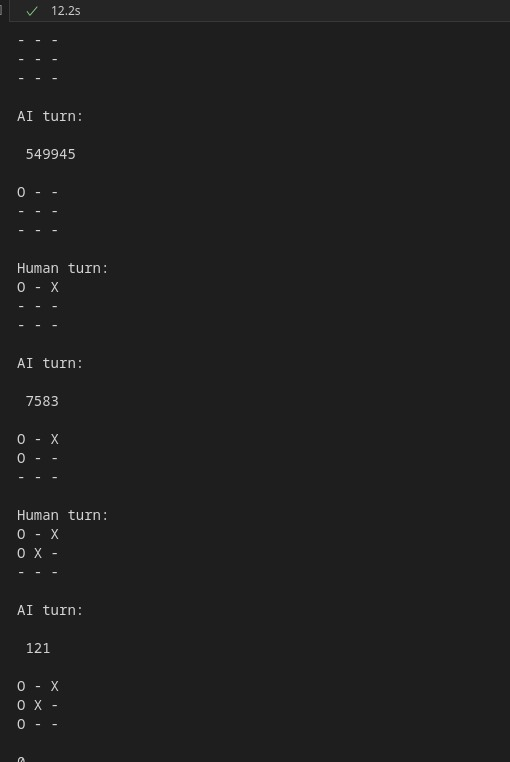
\includegraphics[scale=0.5]{images/4.1.jpg}
\begin{center}
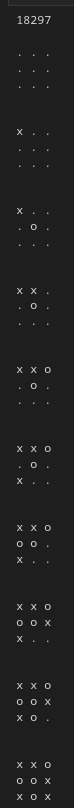
\includegraphics[scale=0.5]{images/4.2.jpg}
\end{center}

\section{Game of Nim}
Each participant in the two-person game of Nim takes turns taking items out of stacks. The goal of the game is to pressure your opponent into picking the final item, leaving them with no options and causing them to lose.\\ \\
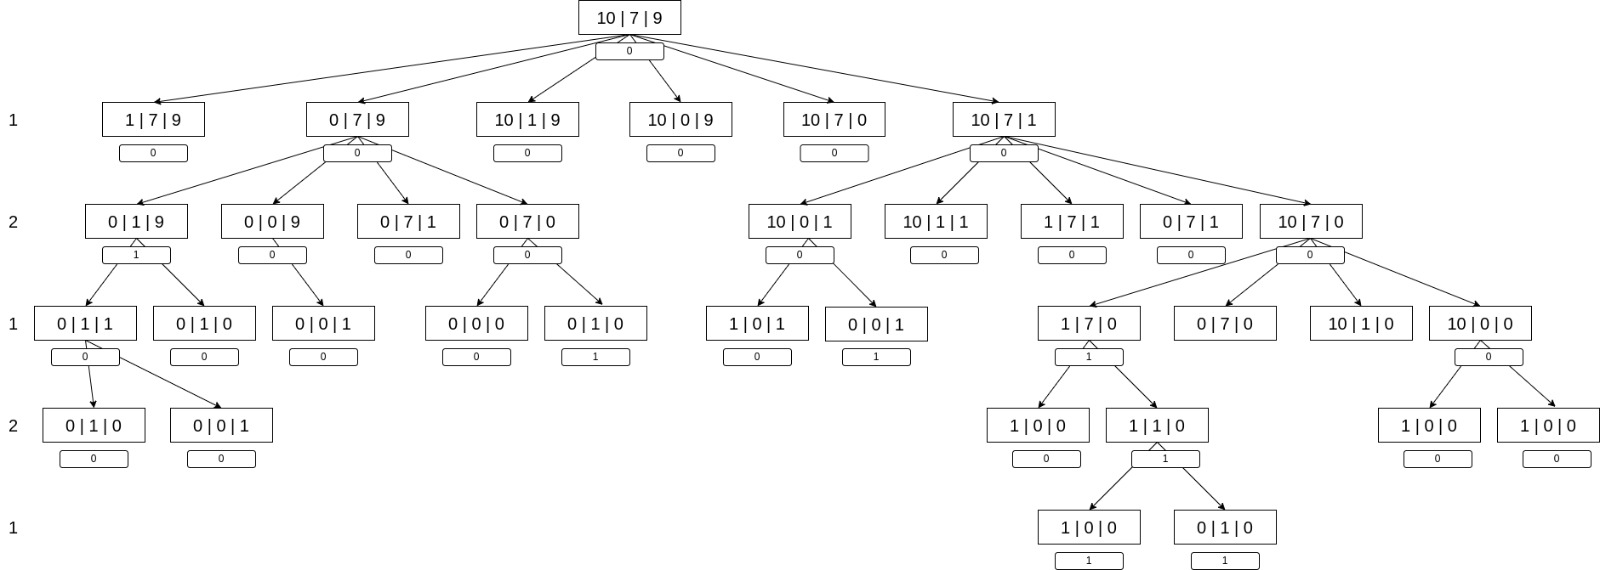
\includegraphics[scale=0.15]{images/4.3.jpg} \\ \\
Thus, Winner is Player 2.
We believe that both players are performing at their best. Then the second player will always win while the first one to move will always lose.\\
To demonstrate this, we examine the initial state to see if the nim total of the piles has a zero xor value.\\
$$10 = 4 + 4 + 2, \quad 7 = 4 + 2 + 1, \quad 9 = 4 + 2 + 2 + 1$$
There are two pairs of (4, 4), two pairs of (2, 2), and one pair of (4, 4). (1, 1). Hence, their XOR value will be 0.\\
Due to the fact that the nim-sum xor is already 0, player 1 cannot make the best move at this time.\\
The player 2 will always prevail if they make moves that result in the nim-sum xor being 0.\\
An instance of Game of Nim is: \\ \\
$(10, 7, 9) \xrightarrow{P1} (10, 7, 5) \xrightarrow{P2} (6, 7, 5) \xrightarrow{P1} (6, 7, 2) \xrightarrow{P2} (6, 4, 2) \xrightarrow{P1} (6, 1, 2) \xrightarrow{P2} (3, 1, 2) \xrightarrow{P1} (1, 1, 2) \xrightarrow{P2} (1, 1, 1) \xrightarrow{P1} (0, 1, 1) \xrightarrow{P2} (0, 1, 0) \xrightarrow{P1} (0,0,0)$ \\ \\
The time complexity for Alpha Beta Pruning would be $O(b^{m/2})$, if it could be done in the most efficient manner.\\
$$T(m) = T(m - 1) + (b - 1) $$
$$T(m - 2) $$
$$T(m) = O(b^{m/2} ) (b^{m/2})$$
This applies to the scenario when we always pick the best node for pruning. The complexity is almost O if we do not select the best move $O(b^{3m/4})$.

\section{Observation}
\indent We found that fewer nodes were reviewed for Alpha Beta Pruning than were evaluated using the Minimax algorithm alone. There are about 10 lakh game trees. Complexity of minimax is $O(b^{m})$ and that of alpha-beta pruning is $O(b^{m/2})$.\\
\indent The nim-sum is necessary for the game of Nim. We must devise a method to ensure that the nim-sum xor is always zero. The winner is the person who achieves nim-sum xor 0. Player 2 will always prevail if the initial state has xor zero; otherwise, Player 1 will prevail. Both athletes were seen to be playing at their best. \\

\section{Conclusion}
We utilised the Minimax algorithm and Alpha Beta pruning to solve the Game of Noughts and Crosses. We see that Alpha Beta Pruning is more effective than the standard Minimax Algorithm. It has been demonstrated that, for the beginning state of the Game of Nim given, player 2 will win every time if player 2 plays well.

\begin{thebibliography}{}
\bibitem{}
 Stuart J. Russell and Peter
Norvig (2022) \emph{Artificial Intelligence - A Modern Approach}, Pearson Education Limited, 4th ed.
\bibitem{}
Tanmay Ambadkar (2021 Artificial Intelligence Course. \href{https://github.com/TanmayAmbadkar/CS302-AI/tree/master/Lab4}{https://github.com/TanmayAmbadkar/CS302-AI/tree/master/Lab4}(2023).
\end{thebibliography}

\end{document}


